Jacobi and Chebyshev smoothers provided rather poor convergence factors for $p$-multigrid with aggressive coarsening.
In this section, we explore using BDDC on single high-order element subdomains as a smoother for $p$-multigrid.

Given the ill-conditioning seen in Figure \ref{fig:lumped_bddc_comparison} for the lumped BDDC preconditioned operator with single high-order element subdomains, we restrict our analysis to Dirichlet BDDC.
As mentioned in Section \ref{sec:fdm_subdomain}, the higher setup cost associated with Dirichlet BDDC for subdomains consisting of multiple low-order elements can be eliminated with the use of FDM approximate solvers for the broken subdomain and subdomain interior problems.

\begin{figure}[!ht]
  \centering
  \subfloat[Lumped BDDC]{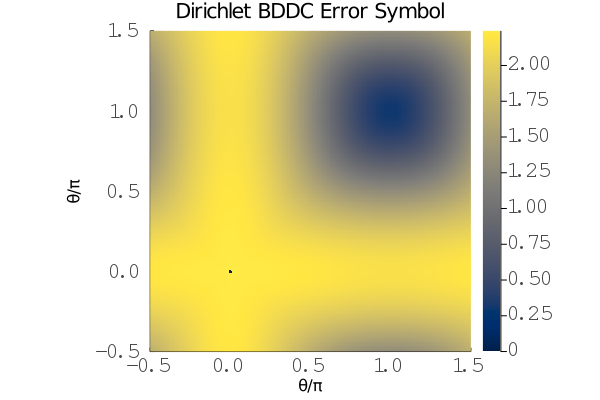
\includegraphics[width=0.48\textwidth]{../img/DirichletBDDCHighOrderNoRelaxation}\label{fig:unrelaxed_bddc}}
  \hfill
  \subfloat[Dirichlet BDDC]{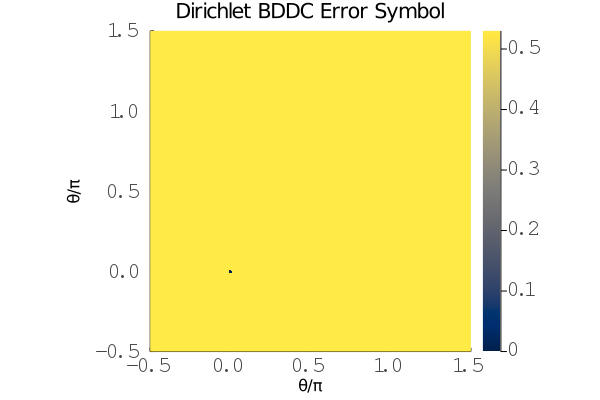
\includegraphics[width=0.48\textwidth]{../img/DirichletBDDCHighOrder47Relaxation}\label{fig:relaxed_bddc}}
  \caption{Symbol of Error Operator for Dirichlet BDDC of 2D Laplacian for $p = 4$}
\end{figure}

In Figure \ref{fig:unrelaxed_bddc} we see the symbol of the error operator for Dirichlet BDDC, given by
\begin{equation}
\tilde{\mathbf{E}} \left( \boldsymbol{\theta} \right) = \mathbf{I} - \tilde{\mathbf{M}}_2^{-1} \tilde{{\color{burgundy}A}} \left( \boldsymbol{\theta} \right),
\end{equation}
for the two dimensional Laplacian
This error operator has a spectral radius greater than one, indicating that the Dirichlet BDDC preconditioner as described above may not be an appropriate smoother for $p$-multigrid.

However, if we introduce a relaxation parameter, $\omega$, as used in the Jacobi preconditioner, then we see an improved spectral radius in Figure \ref{fig:relaxed_bddc} for the error operator.
The symbol of the error operator with a relaxation parameter is given by
\begin{equation}
\tilde{\mathbf{E}} \left( \boldsymbol{\theta}, \omega \right) = \mathbf{I} - \omega \tilde{\mathbf{M}}_2^{-1} \tilde{{\color{burgundy}A}} \left( \boldsymbol{\theta} \right).
\end{equation}

\begin{table}[ht!]
\begin{center}
\begin{tabular}{l cc}
  \toprule
  $p_{\text{fine}}$ to $p_{\text{coarse}}$  & $\rho_{\min}$ & $\omega_{\text{opt}}$  \\
  \toprule
  $p = 2$ to $p = 1$   &  0.121 & 0.66  \\
  \midrule
  $p = 4$ to $p = 2$   &  0.272 & 0.48  \\
  $p = 4$ to $p = 1$   &  0.281 & 0.47  \\
  \midrule
  $p = 8$ to $p = 4$   &  0.409 & 0.38  \\
  $p = 8$ to $p = 2$   &  0.462 & 0.33  \\
  $p = 8$ to $p = 1$   &  0.462 & 0.32  \\
  \midrule
  $p = 16$ to $p = 8$  &  0.504 & 0.32  \\
  $p = 16$ to $p = 4$  &  0.579 & 0.25  \\
  $p = 16$ to $p = 2$  &  0.597 & 0.23  \\
  $p = 16$ to $p = 1$  &  0.597 & 0.23  \\
  \bottomrule
\end{tabular}
\end{center}
\caption{Two-Grid Convergence Factor for $p$-Multigrid with BDDC Smoother for 2D Laplacian}
\label{table:two_grid_bddc_smoother}
\end{table}

In Table \ref{table:two_grid_bddc_smoother}, we see the two-grid convergence factor for $p$-multigrid with the weighted Dirichlet BDDC smoother for the two dimensional Laplacian.
When compared to Table \ref{table:two_grid_2d_chebyshev}, we can see that the weighted Dirichlet BDDC smoother provides a significantly improved two-grid convergence factor for aggressive coarsening with high-order elements when compared to fourth order Chebyshev smoothing.
Additionally, the weighted Dirichlet BDDC smoother provides analogous two-grid convergence factors when compared to more conservative coarsening strategies with second or third order Chebyshev smoothing.

Even when Dirichlet BDDC smoothing provides analogous convergence factors to third or fourth order Chebyshev smoothing, the Dirichlet BDDC smoother offers benefits in global communication requirements.
A $k$th order Chebyshev smoother requires $k$ full operator evaluations, each of which requires global communication.
In contrast, the application of the Dirichlet BDDC smoother requires two applications of the subassembled operator on the primal space, one solve of the Schur complement on the primal space, and the global communication from the transpose injection operation.
The primal space is significantly smaller than the global problem, which means that much less communication is required to apply the Dirichlet BDDC smoother compared to a third or fourth order Chebyshev smoother.

\begin{table}[ht!]
\begin{center}
\begin{tabular}{l cc}
  \toprule
  $p_{\text{fine}}$ to $p_{\text{coarse}}$  & $\rho_{\min}$ & $\omega_{\text{opt}}$  \\
  \toprule
  $p = 2$ to $p = 1$   &  0.601 & 0.25  \\
  \midrule
  $p = 3$ to $p = 2$   &  0.723 & 0.15  \\
  $p = 3$ to $p = 1$   &  0.723 & 0.15  \\
  \midrule
  $p = 4$ to $p = 3$   &  0.903 & 0.05  \\
  $p = 4$ to $p = 2$   &  0.903 & 0.05  \\
  $p = 4$ to $p = 1$   &  0.903 & 0.05  \\
  \midrule
  $p = 8$ to $p = 4$   &  0.980 & 0.01  \\
  $p = 8$ to $p = 2$   &  0.980 & 0.01  \\
  $p = 8$ to $p = 1$   &  0.980 & 0.01  \\
  \bottomrule
\end{tabular}
\end{center}
\caption{Two-Grid Convergence Factor for $p$-Multigrid with BDDC Smoother for 3D Laplacian}
\label{table:two_grid_bddc_smoother_3d}
\end{table}

In Table \ref{table:two_grid_bddc_smoother_3d}, we see the two-grid convergence factor for $p$-multigrid with the weighted Dirichlet BDDC smoother for the three dimensional Laplacian.
As anticipated, a primal space consisting only of element vertices on the corners in three dimensions is inadequate for fourth-order or higher elements.
Technically, a Richardson iteration with fourth-order or eight-order elements with the weighting factors given above will converge, but as seen in Table \ref{table:error_tolerance}, this iteration will converge very slowly.
However, a vertex only primal space is still sufficient for cubic and quadratic elements.
